\chapter{Introduction}

Signal processing has long relied on well-defined, structured processes and protocols to function.  
However, in order to move towards more robust and adaptive systems, we will need to overhaul these tightly structured processes.  We must design new robust and adaptive communications systems.

From an academic perspective, the rise of machine learning tools and processing has allowed us to tackle problems we have not yet been able to, like in image processing.  However, we still do not fully understand the possibilities or the limitations of this technology.  
Most applications for machine learning techniques lack good baselines to compare performance.
Applications such as image processing \cite{imagenet}, videogame control \cite{videogame}, playing the game Go, \cite{alphago}, and natural language processing \cite{nlp}, are all missing good baselines to compare against.
In order to study the limitations of machine learning techniques, we must apply them to spaces that we have studied extensively, like communications, and compare them to the well-known baselines that are already very good.

Most communications systems have three main processes at the receiver; equalization, demodulation, and error-correction.  While we will need to design robust forms of all of these processes, we will focus on equalization for the remainder of this report. 

\section{Motivation}

Meta-learning is the idea that algorithms need to be able to `learn to learn' in order to generalize to different applications.  For example, if a robot is trained to pick up coffee mugs, then we want that robot to be able to quickly learn how to pick up water bottles without having to re-train the robot.  
Meta-learning is inspired by humans ability to generalize how to learn \cite{lake}.  
Additionally, researchers in neurology have studied how the brain synapses change over time, suggesting that our algorithms will have to change over time to continue learning \cite{bengio}.
Our brains know how to update the synapses as we learn new things. This is like updating the weights of a neural network for new data points.  
We refer the reader to \cite{lemke} for a survey of meta-learning technologies and to \cite{finn} for recent developments in meta-learning algorithms.

In this report, we want to understand if our neural network based communication processes can learn to learn.  
As in, can they handle new environments with new data sequeneces without having to re-train for the new variables. 
The communications application is arguably an easier application of meta-learning than others have been exploring, like image classification \cite{khodadadeh}.  
In order to better understand the possibilities and limitations of meta-learning, we need to apply it to something simpler, like communications.  In this report, we will explore whether or not we can learn to learn to communicate. 

\subsection{Context}

A team at UC Berkeley and Nokia Bell Labs  participated in the DARPA Spectrum Collaboration Challenge, a competition to build collaborative, intelligent radios\footnote{I was heavily involved with this project and this report grew out of my work on this challenge.}.
The challenge consists of putting multiple radio networks in the same space and bandwidth.  
Without having been codesigned, the networks must collaborate and share all of the resources.
The environment was open to all of the teams so there are no rigid bands like we use today.

One of the potential scenarios for this challenge was that networks might have stranded radios where no radio in their own network can reach them.  In this case, that network would need to rely on another network to relay messages to and from the stranded node.  
The challenge is that the relay network must forward along a signal that it cannot fully decode itself.  This requires the network to equalize a signal and correct for CFO and then send it without using demodulation or error-correction.  
This challenge is one of the practical applications for robust and adaptive processes for equalization.

\section{Background}

While we will not be designing new modulation or demodulation processes in this report, we must introduce some terminology.
A constellation is a mapping of bits to complex symbols.  
A classic quadrature phase shift keying (QPSK) modulator maps pairs of bits to complex symbols.
For the remainder of the report, when we use a QPSK constellation, we use the following mapping.
\begin{align*}
\begin{bmatrix}
\text{Bits} & \text{Complex Symbol} \\
\hline
00 & -1-1j \\
10 & 1 -1j \\
01 & -1 + 1j \\
11 & 1+1j \\
\end{bmatrix}
\end{align*}

We will also use signal to noise ratio (SNR) to evaluate our models.  SNR is the ratio of the signal power to the noise power.  
If the SNR is greater than one, then this means that there is more signal than noise.  If the SNR is infinity, this means that there is no noise added.
We use $\text{SNR}=\frac{E_b}{N_0}$ where $E_b$ is the energy per bit and $N_0$ is the noise power spectral density.
We set the SNR in our simulations by changing the noise power of a Gaussian random variable. 

\subsection{Inter-symbol Interference and Equalization}

Inter-symbol interference occurs when we are transmitting over a channel that has some echos.  These echos cause the receiver to hear a garbled signal instead of the original signal from the transmitter.  This is called inter-symbol interference because the receiver is hearing a combination of symbols across time. 

Let $\vec{x}=[x_0, x_1, \ldots x_n]$ be the set of $n$ complex symbols that the transmitter sends over the channel that connects the transmitter to the receiver.
Each channel will have different characteristics. Some channels may have echos, others may have delays, often channels will have both.  When a channel has echos, this is called a multipath channel because there are multiple paths to reach the receiver.  
When a channel is modeled as a delay line, each multipath signal component at the receiver is modeled as a tap on the delay line.  
We can characterize a channel by characterizing the channel taps.

Let $\vec{a} = [a_0, a_1, \ldots a_{\ell}]$ be the characteristics for a multipath channel that has $\ell+1$ taps. When a sequence of symbols like $\vec{x}$ is transmitted over this channel, the channel taps are convolved over the sequence.  Additionally, there is noise in the system denoted by $v_m$. 

\begin{align}
\tilde{x}_m = \sum_{i=0}^{\ell} a_i x_{m-i} + v_m
\end{align}

The receiver will hear a signal that is corrupted by inter-symbol interfence and noise;
$\vec{\tilde{x}}=[\tilde{x}_0, \tilde{x_1}, \ldots \tilde{x}_{n+\ell}]$. 
Receivers must be able to handle garbled signals in order to transmit data in the real world.  The process of removing the inter-symbol interference is called equalization.  The goal of equalization is to take in a garbled signal and output a signal with minimal inter-symbol interference. 

Figure~\ref{fig:multi_tap} demonstrates the effects of two tap channels on a QPSK modulation constellation.  
We show what the received signal constellations are from a sequence of $100$ symbols modulated in QPSK through different two tap channels.  The channel taps are normalized, $||\vec{a}||^2=1$.  We assume that the channel taps are constant during the transmission of the signal.
We see that under certain channel conditions, like when the two taps are equal, it is very difficult to distinguish between the four constellations.  
We also show how the constellations change with lower SNR.  When the SNR is infinity, i.e. when no noise is added, the first and third channel constellations are distinct and clear.  However, as we add noise (lower SNR), the symbol groupings get mixed and there are less clear distinctions between the symbols.
Engineers have built processes to remove inter-symbol interference.  First, let's go into the case when the channel characteristics are known.

\setlength{\tabcolsep}{0pt}
\begin{figure}
  \centering
  \caption{The effects of a two tap channel on the QPSK constellation.}
  \begin{tabular}{ccc}
    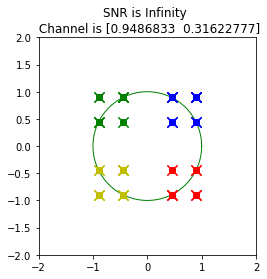
\includegraphics[width=45mm]{figures/equal_intro/snr_0_c3/cfo_0.png}&
    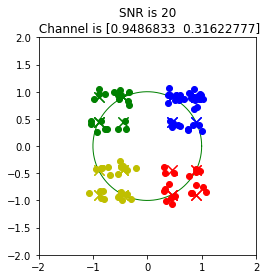
\includegraphics[width=45mm]{figures/equal_intro/snr_20_c3/cfo_0.png}&
    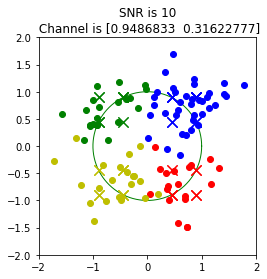
\includegraphics[width=45mm]{figures/equal_intro/snr_10_c3/cfo_0.png}\\
    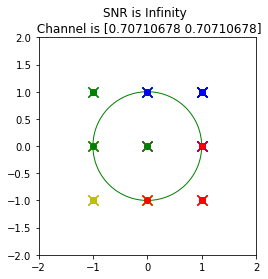
\includegraphics[width=45mm]{figures/equal_intro/snr_0_c2/cfo_0.png}&
    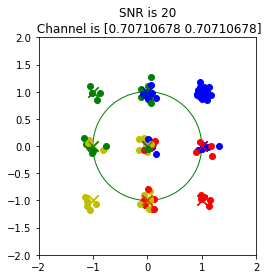
\includegraphics[width=45mm]{figures/equal_intro/snr_20_c2/cfo_0.png}&
    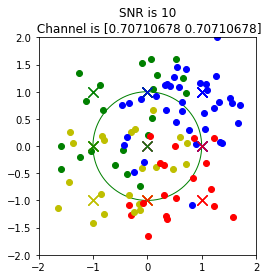
\includegraphics[width=45mm]{figures/equal_intro/snr_10_c2/cfo_0.png}\\
    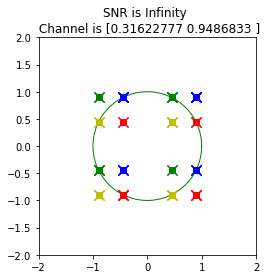
\includegraphics[width=45mm]{figures/equal_intro/snr_0_c4/cfo_0.png}&
    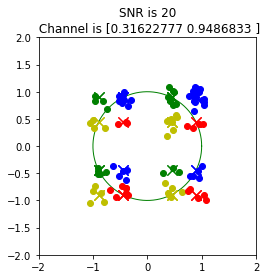
\includegraphics[width=45mm]{figures/equal_intro/snr_20_c4/cfo_0.png}&
    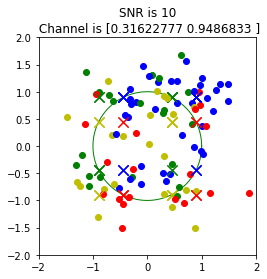
\includegraphics[width=45mm]{figures/equal_intro/snr_10_c4/cfo_0.png}\\
    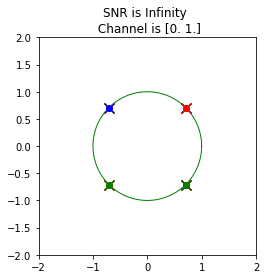
\includegraphics[width=45mm]{figures/equal_intro/snr_0_c5/cfo_0.png}&
    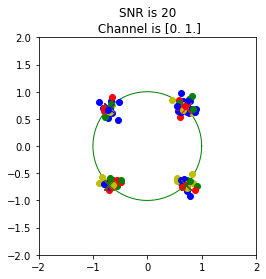
\includegraphics[width=45mm]{figures/equal_intro/snr_20_c5/cfo_0.png}&
    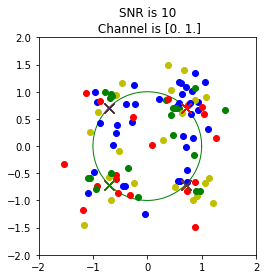
\includegraphics[width=45mm]{figures/equal_intro/snr_10_c5/cfo_0.png}\\
  \end{tabular}
  \label{fig:multi_tap}
\end{figure}

\subsubsection{Equalization for a known channel}

If the receiver knows the channel characteristics, $\vec{a}$, perfectly, then there are a few different methods that can be used.  
The zero-forcing equalizer applies the inverse of the channel response to the received signal.  It is called zero-forcing because there will be zero inter-symbol interference if there is no noise.
There are some limitations of the zero-forcing equalizer. 
First, the impulse response of the equalizer needs to be infinitely long. 
Second, if there is a weak signal at a frequency, then the inverse gain is going to be very large.  This will amplify any noise in the system. 
Third, if there are any zeros in the frequency response, these cannot be inverted.

Another equalizer, the minimum mean squared error (MMSE) equalizer, handles noise much better than the zero-forcing equalizer.
The MMSE equalizer minimizes the error between the equalized preamble and the original known preamble by choosing the optimal inverse of the channel response, $W$.  Let $H$ be the circulant matrix of the channel taps.
\begin{align}
\vec{\tilde{x}}_{pre} &= H\vec{x}_{pre}+\vec{v}\\ 
H &= \begin{bmatrix}
a_0 & 0 & & & \cdots & & 0 \\
a_1 & a_0 & 0 & & \cdots & & 0 \\
\vdots & & & & & & \vdots \\
a_{\ell} & a_{\ell-1} & \cdots & a_0 & 0 & \cdots & 0 \\
0 & a_{\ell} & a_{\ell-1} & \cdots & a_0 & \cdots & 0 \\
\vdots & & & & & & \vdots \\
0 & \cdots & 0 & a_{\ell} & a_{\ell-1} & \cdots & a_0 \\
\end{bmatrix}\\
& \min_W||\vec{x}_{pre}-\vec{\hat{x}}_{pre}||^2 \\
\vec{\hat{x}}_{pre} &= W (H\vec{x}_{pre}+\vec{v}) \\
W^* &= \vec{x}_{pre} \vec{x}_{pre}^T H^T (H \vec{x}_{pre} \vec{x}_{pre}^T H^T + \sigma_v^2 I)^{-1}
\end{align}

The MMSE equalizer works well for known and unknown channels and does not amplify noise like the zero-forcing equalizer.
While it is important to consider how well a receiver can equalize with a known channel, this is rarely the case.  Usually, we do not know the channel characteristics.

\subsubsection{Equalization for an unknown channel}
When the receiver does not know the channel characteristics, the process of equalization essentially has two jobs; first, identify the channel, second, remove the inter-symbol interference. If the receiver did not identify the channel first, there would be no way to remove the effects of it on the received signal. 

In order to estimate a channel, most systems require that packets begin with a known sequence called a preamble. The signal sent is broken into two parts; $\vec{x} = [\vec{x}_{pre}, \vec{x}_{data}]$.  The signal received on the transmitter is $\vec{\tilde{x}}=[\vec{\tilde{x}}_{pre},\vec{\tilde{x}}_{data}]$.  
The receiver knows what the orginal preamble sequence was, $\vec{x}_{pre}$, and can use the received preamble sequence, $\vec{\tilde{x}}_{pre}$, to estimate the behavior of the channel.
Once the channel is estimated, the receiver then equalizes the data, $\vec{\tilde{x}}_{data}$.

One common method to estimate the channel is to use the least-squares optimization framework. Let $H$ be the circulant matrix of estimates of the channel taps.  The least-squares channel estimator wants to find $H$ that minimizes the mean squared error between the received signal, $\vec{\tilde{x}}_{pre}$, and what the predicted received signal would be if the the estimated channel $H$ were applied to the original preamble, $\vec{x}_{pre}$.
\begin{align}
\min_H ||\vec{\tilde{x}}_{pre}-H\vec{x}_{pre}||^2
\end{align}

The receiver needs to choose the number of non-zeros in $H$, representing how many taps (or echos) there might be in the channel.  The number of taps, or non-zeros, in $H$ will be set based on the environment of the transmitter and receiver.
Once the channel response has been estimated, an equalizer uses that information to remove the inter-symbol interference from the received signal, like the MMSE equalizer defined above.

 
\subsection{Carrier Frequency Offset and Correction}

If we were to implement our minimum mean squared error equalizer on a real-world physical receiver, we would find some problems with our equalization process.  
Our equalizer will equalize the first symbols very well.  However, as we equalize later parts of our sequence, we will encounter a physical phenomonen called carrier frequency offset, CFO.
Carrier frequency offset can occur when the transmitter and receiver are at slightly different frequencies.  It can also occur when the transmitter and receiver are moving, causing a sort of Doppler effect. 

When there is a significant CFO present, the symbols will gradually rotate. The received signals will be the original signals rotated at a rate $\omega$. Gaussian noise, $v_m$, is also added.
\begin{align}
\tilde{x}_m = x_m e^{mj\omega}+v_m
\end{align} 

Figure~\ref{fig:single_tap_cfo} demonstrates the effects of pure CFO on a QPSK modulation constellation (no multipath). 
We show what the received signal symbols constellations are from a sequence of $100$ symbols modulated in QPSK with different CFO rates.  We assume that the CFO rate, $\omega$, is constant during the transmission of the signal.
For small CFO rates, the data does not rotate that much.  For larger CFO rates, the data turns more and as we add noise (lower SNR), the groupings of the symbols become mixed.

\setlength{\tabcolsep}{0pt}
\begin{figure}
  \centering
  \caption{The effects of a carrier frequency offset on the QPSK constellation.}
  \begin{tabular}{ccc}
    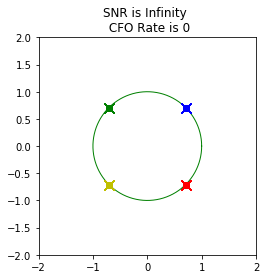
\includegraphics[width=50mm]{figures/cfo_intro/snr_0/cfo_0.png}&
    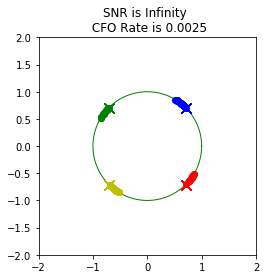
\includegraphics[width=50mm]{figures/cfo_intro/snr_0/cfo_1.png}&
    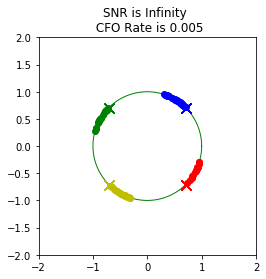
\includegraphics[width=50mm]{figures/cfo_intro/snr_0/cfo_2.png}\\
    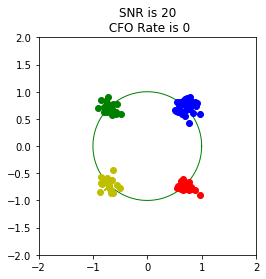
\includegraphics[width=50mm]{figures/cfo_intro/snr_20/cfo_0.png}&
    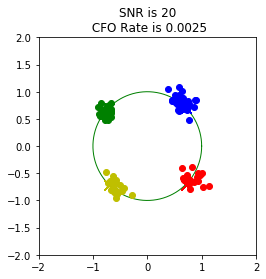
\includegraphics[width=50mm]{figures/cfo_intro/snr_20/cfo_1.png}&
    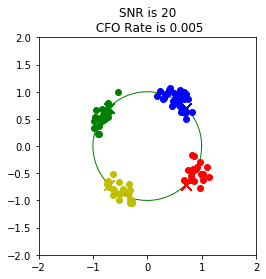
\includegraphics[width=50mm]{figures/cfo_intro/snr_20/cfo_2.png}\\
    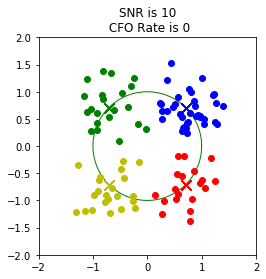
\includegraphics[width=50mm]{figures/cfo_intro/snr_10/cfo_0.png}&
    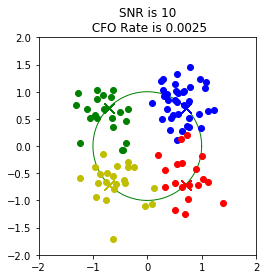
\includegraphics[width=50mm]{figures/cfo_intro/snr_10/cfo_1.png}&
    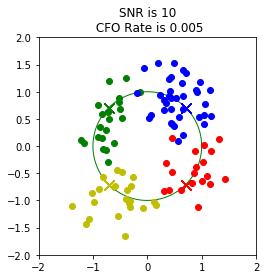
\includegraphics[width=50mm]{figures/cfo_intro/snr_10/cfo_2.png}
  \end{tabular}
  \label{fig:single_tap_cfo}
\end{figure}

There are a few ways to handle CFO, some are more elegant than others. 
The first solution is to try to side-step the problem entirely.  
Since the effects of CFO depend on the length of a packet, one solution is to make packets so short that the symbols only move a little bit.  In this case, the effects of CFO can be ignored.

Another solution is using a phase-locked loop, which is a control system that outputs a signal with a phase related to the input signal.  
A Costas loop is a circuit that implements a phase-locked loop for CFO correction for continuous time signals by adapting the sampling rate \cite{costas}.  
However, this requires adjusting the sampling and is implemented in hardware.  This does not allow the robustness and adaptability that we want.

What happens when there is both CFO and inter-symbol interference?  The received signal will have the effects of the channel and CFO as well as the noise. 

\begin{align}
\tilde{x}_m = (\sum_{i=0}^{\ell} a_i x_{m-i})e^{mj\omega} + v_m
\end{align}

Figure~\ref{fig:multi_tap_cfo} demonstrates the effects of CFO and multi-tap channels on a QPSK modulation constellation. 
We show what the received signal symbols constellations are from a sequence of $100$ symbols modulated in QPSK with different CFO rates and two tap channels.  We assume that the CFO rate, $\omega$, and the channel taps are constant during the transmission of the signal.  
The channel taps are normalized, $||\vec{a}||^2=1$ for each of the channels. 
We can see that for certain channel conditions, like for the channel in the third row, that the combination of carrier frequency offset and noise makes grouping these symbols quite difficult. 
Modern day receivers have to combine CFO correction, channel estimation, and equalization processes in order to handle these received signals.

\setlength{\tabcolsep}{0pt}
\begin{figure}
  \centering
  \caption{The effects of a two tap channel and a carrier frequency offset on the QPSK constellation.}
  \begin{tabular}{ccc}
    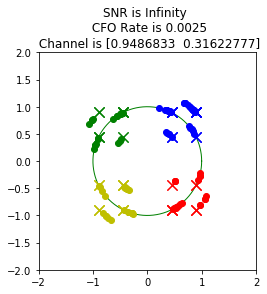
\includegraphics[width=45mm]{figures/cfo_equal_intro/snr_0_c3/cfo_0.png}&
    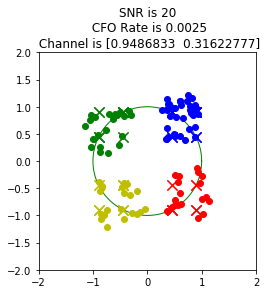
\includegraphics[width=45mm]{figures/cfo_equal_intro/snr_20_c3/cfo_0.png}&
    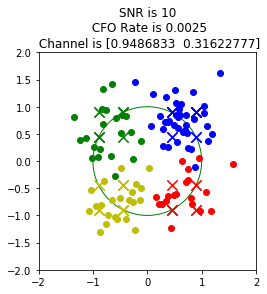
\includegraphics[width=45mm]{figures/cfo_equal_intro/snr_10_c3/cfo_0.png}\\
    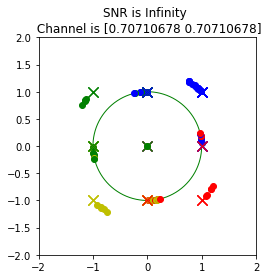
\includegraphics[width=45mm]{figures/cfo_equal_intro/snr_0_c2/cfo_0.png}&
    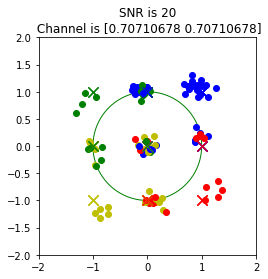
\includegraphics[width=45mm]{figures/cfo_equal_intro/snr_20_c2/cfo_0.png}&
    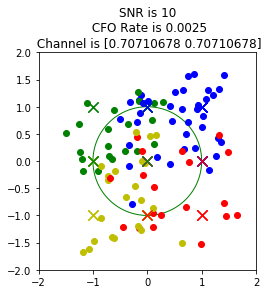
\includegraphics[width=45mm]{figures/cfo_equal_intro/snr_10_c2/cfo_0.png}\\
    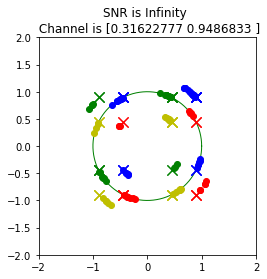
\includegraphics[width=45mm]{figures/cfo_equal_intro/snr_0_c4/cfo_0.png}&
    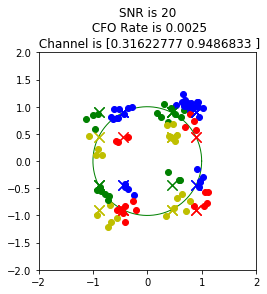
\includegraphics[width=45mm]{figures/cfo_equal_intro/snr_20_c4/cfo_0.png}&
    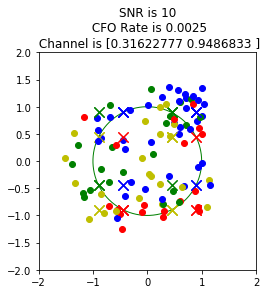
\includegraphics[width=45mm]{figures/cfo_equal_intro/snr_10_c4/cfo_0.png}\\
    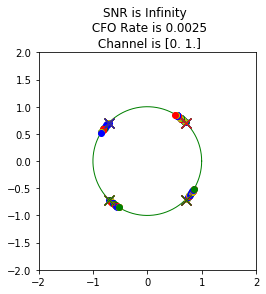
\includegraphics[width=45mm]{figures/cfo_equal_intro/snr_0_c5/cfo_0.png}&
    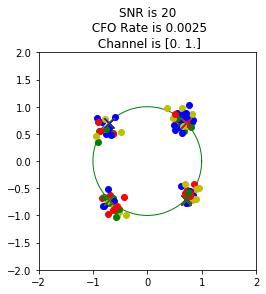
\includegraphics[width=45mm]{figures/cfo_equal_intro/snr_20_c5/cfo_0.png}&
    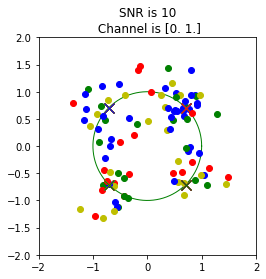
\includegraphics[width=45mm]{figures/cfo_equal_intro/snr_10_c5/cfo_0.png}\\
  \end{tabular}
  \label{fig:multi_tap_cfo}
\end{figure}

\section{Related Works}

related works!


\cite{dorner2017}

\cite{kim2018}

\cite{farsad2018}

\cite{osheacsi}

\cite{diamandis}

\cite{raghavendra}

\cite{botoca}

\cite{ye2018}

\cite{osheamimo}

\cite{wang}

\cite{kimnips}

\cite{finn}

\cite{lake}

\cite{osheavoid}

\cite{yegans}

\cite{hemodel}

\cite{osheasynch}

\section{Contributions of this Report}

In this report, we show that a channel estimator can learn to learn to estimate two tap, real-valued channels but that more work is needed for the network to perform comparably to the baseline, the least-squares channel estimator.
We also design an equalizer recursive neural network that equalizes a stream of data for any two tap, real-valued channel. This equalizer does not need to re-train for each new channel and performs better than the baseline, the minimum mean squared error equalizer, for low signal to noise ratios.  We also show that the baseline is much better than the neural network at handling difficult channels, specifically channels that have approximately equal taps.

This work is novel in this area because all of the other related works have re-trained the networks for each new channel they encounter.  This is the first equalizer that learns to learn to handle each new channel without having to re-train. Table~\ref{tab:table1} compares our work with previous works.

\setlength{\tabcolsep}{4pt}
\begin{table}[h!]
  \begin{center}
    \caption{Comparison of our work and related works.}
    \label{tab:table1}
    \begin{tabular}{c|c|c|c|c} % <-- Alignments: 1st column left, 2nd middle and 3rd right, with vertical lines in between
       & {Goldsmith \cite{farsad2018}} & {Ye \cite{ye2018}} & {O'Shea \cite{osheaatt}} & {Our Work}\\
      \hline
      Types of channels & Poisson & AWGN & AWGN &AWGN \\
           considered &  & Multipath & Multipath & Multipath\\
           \hline
      Do they address CFO? & No & No & Yes & Yes \\
      \hline
      Do they re-train for & No & Yes & No & No\\
      each new enviornment? &  &  &  &\\
    \end{tabular}
  \end{center}
\end{table}

Additionally, we design a neural network to estimate and correct carrier frequency offset that does not need to be retrained for each new carrier frequency offset.
This work is novel in this area because the other related works have re-trained the networks for each new carrier frequency offset.  This is the first carrier frequency offset correction network that learns to learn to handle each new carrier frequency offset without having to re-train.
We also explore whether recursive neural networks can behave as clocks and show that this is a non-trivial problem that needs more exploration.
